\documentclass[12pt, a4paper, oneside, openright, titlepage]{book}
\usepackage[utf8]{inputenc}
\raggedbottom
%%%%%%%%%%%%%%%%% Book Formatting Comments:

%%%%%%%%%%%%%%%%%%%%%%%%%%%%%%%%%%%%% for Part

%%%%%%%%%%%%%%%%%%%%%% for chapter

%%%%%%%%%%%%%%%%%%%% for section




%%%%%% PACKAGES %%%%%%%
\usepackage{hyperref}
\hypersetup{
    colorlinks,
    citecolor=black,
    filecolor=black,
    linkcolor=black,
    urlcolor=black
}
\usepackage{amsmath} % Math display options
\usepackage{amssymb} % Math symbols
%\usepackage{amsfonts} % Math fonts
%\usepackage{amsthm}
\usepackage{mathtools} % General math tools
\usepackage{array} % Allows you to write arrays
\usepackage{empheq} % For boxing equations
% \usepackage{mathabx}
% \usepackage{mathrsfs}
\usepackage{nameref}
\usepackage{wrapfig}

\usepackage{soul}
\usepackage[normalem]{ulem}

\usepackage{txfonts}
\usepackage{cancel}
\usepackage[toc, page]{appendix}
\usepackage{titletoc,tocloft}
\setlength{\cftchapindent}{1em}
\setlength{\cftsecindent}{2em}
\setlength{\cftsubsecindent}{3em}
%\setlength{\cftsubsubsecindent}{4em}
\usepackage{titlesec}

%\titleformat{\section}
%  {\normalfont\fontsize{25}{15}\bfseries}{\thesection}%{1em}{}
%\titleformat{\section}
%  {\normalfont\fontsize{20}{15}\bfseries}%{\thesubsection}{1em}{}
%\setcounter{secnumdepth}{1}  
  
  

%\newcommand\numberthis{\refstepcounter{equation}\tag{\theequation}} % For equation labelling
\usepackage[framemethod=tikz]{mdframed}

\usepackage{tikz} % For drawing commutative diagrams
\usetikzlibrary{cd}
\usetikzlibrary{calc}
\tikzset{every picture/.style={line width=0.75pt}} %set default line width to 0.75p

\usepackage{datetime}
\usepackage[margin=1.5in]{geometry}
\setlength{\parskip}{1em}
\usepackage{makeidx}         % allows index generation
\usepackage{graphicx}       % standard LaTeX graphics tool
\usepackage{multicol}        % used for the two-column index
\usepackage[bottom]{footmisc}% places footnotes at page bottom

\usepackage{newtxtext}       % 
\usepackage{newtxmath}       % selects Times Roman as basic font
\usepackage{float}
\usepackage{fancyhdr}
\setlength{\headheight}{15pt} 
\pagestyle{fancy}
\lhead[\leftmark]{}
\rhead[]{\leftmark}

%\usepackage{enumitem}

\usepackage{url}
\allowdisplaybreaks

%%%%%% ENVIRONMENTS %%%
\definecolor{purp}{rgb}{0.29, 0, 0.51}
\definecolor{bloo}{rgb}{0, 0.13, 0.80}



%%\newtheoremstyle{note}% hnamei
%{3pt}% hSpace above
%{3pt}% hSpace belowi
%{}% hBody fonti
%{}% hIndent amounti
%{\itshape}% hTheorem head fonti
%{:}% hPunctuation after theorem headi
%{.5em}% hSpace after theorem headi
%{}% hTheorem head spec (can be left empty, meaning ‘normal’)i





% %%%%%%%%%%%%% THEOREM DEFINITIONS

\spnewtheorem{axiom}{Axiom}[chapter]{\bfseries}{\itshape}


\spnewtheorem{construction}{Construction}[chapter]{\bfseries}{\itshape}

\spnewtheorem{props}{Properties}[chapter]{\bfseries}{\itshape}


\renewcommand{\qedsymbol}{$\blacksquare$}


\numberwithin{equation}{section}

\newenvironment{qest}{
    \begin{center}
        \em
    }
    {
    \end{center}
    }

%%%%%% MACROS %%%%%%%%%
%% New Commands
\newcommand{\ip}[1]{\langle#1\rangle} %%% Inner product
\newcommand{\abs}[1]{\lvert#1\rvert} %%% Modulus
\newcommand\diag{\operatorname{diag}} %%% diag matrix
\newcommand\tr{\mbox{tr}\.} %%% trace
\newcommand\C{\mathbb C} %%% Complex numbers
\newcommand\R{\mathbb R} %%% Real numbers
\newcommand\Z{\mathbb Z} %%% Integers
\newcommand\Q{\mathbb Q} %%% Rationals
\newcommand\N{\mathbb N} %%% Naturals
\newcommand\F{\mathbb F} %%% An arbitrary field
\newcommand\ste{\operatorname{St}} %%% Steinberg Representation
\newcommand\GL{\mathbf{GL}} %%% General Linear group
\newcommand\SL{\mathbf{SL}} %%% Special linear group
\newcommand\gl{\mathfrak{gl}} %%% General linear algebra
\newcommand\G{\mathbf{G}} %%% connected reductive group
\newcommand\g{\mathfrak{g}} %%% Lie algebra of G
\newcommand\Hbf{\mathbf{H}} %%% Theta fixed points of G
\newcommand\X{\mathbf{X}} %%% Symmetric space X
\newcommand{\catname}[1]{\normalfont\textbf{#1}}
\newcommand{\Set}{\catname{Set}} %%% Category set
\newcommand{\Grp}{\catname{Grp}} %%% Category group
\newcommand{\Rmod}{\catname{R-Mod}} %%% Category r-modules
\newcommand{\Mon}{\catname{Mon}} %%% Category monoid
\newcommand{\Ring}{\catname{Ring}} %%% Category ring
\newcommand{\Topp}{\catname{Top}} %%% Category Topological spaces
\newcommand{\Vect}{\catname{Vect}_{k}} %%% category vector spaces'
\newcommand\Hom{\mathbf{Hom}} %%% Arrows

\newcommand{\map}[2]{\begin{array}{c} #1 \\ #2 \end{array}}

\newcommand{\Emph}[1]{\textbf{\ul{\emph{#1}}}}




%% Math operators
\DeclareMathOperator{\ran}{Im} %%% image
\DeclareMathOperator{\aut}{Aut} %%% Automorphisms
\DeclareMathOperator{\spn}{span} %%% span
\DeclareMathOperator{\ann}{Ann} %%% annihilator
\DeclareMathOperator{\rank}{rank} %%% Rank
\DeclareMathOperator{\ch}{char} %%% characteristic
\DeclareMathOperator{\ev}{\bf{ev}} %%% evaluation
\DeclareMathOperator{\sgn}{sign} %%% sign
\DeclareMathOperator{\id}{Id} %%% identity
\DeclareMathOperator{\supp}{Supp} %%% support
\DeclareMathOperator{\inn}{Inn} %%% Inner aut
\DeclareMathOperator{\en}{End} %%% Endomorphisms
\DeclareMathOperator{\sym}{Sym} %%% Group of symmetries


%% Diagram Environments
\iffalse
\begin{center}
    \begin{tikzpicture}[baseline= (a).base]
        \node[scale=1] (a) at (0,0){
          \begin{tikzcd}
           
          \end{tikzcd}
        };
    \end{tikzpicture}
\end{center}
\fi




\newdateformat{monthdayyeardate}{%
    \monthname[\THEMONTH]~\THEDAY, \THEYEAR}
%%%%%%%%%%%%%%%%%%%%%%%

\newcommand{\mb}[1]{\mathbf{#1}}

%%%%%% BEGIN %%%%%%%%%%


\begin{document}

%%%%%% TITLE PAGE %%%%%

\begin{titlepage}
    \centering
    \scshape
    \vspace*{\baselineskip}
    \rule{\textwidth}{1.6pt}\vspace*{-\baselineskip}\vspace*{2pt}
    \rule{\textwidth}{0.4pt}
    
    \vspace{0.75\baselineskip}
    
    {\LARGE Linear Algebra: A complete Guide}
    
    \vspace{0.75\baselineskip}
    
    \rule{\textwidth}{0.4pt}\vspace*{-\baselineskip}\vspace{3.2pt}
    \rule{\textwidth}{1.6pt}
    
    \vspace{2\baselineskip}
    Linear Algebra \\
    \vspace*{3\baselineskip}
    \monthdayyeardate\today \\
    \vspace*{5.0\baselineskip}
    
    {\scshape\Large Elijah Thompson, \\ Physics and Math Honors\\}
    
    \vspace{1.0\baselineskip}
    \textit{Solo Pursuit of Learning}
    \vfill
    \enlargethispage{1in}
    \begin{figure}[b!]
    \makebox[\textwidth]{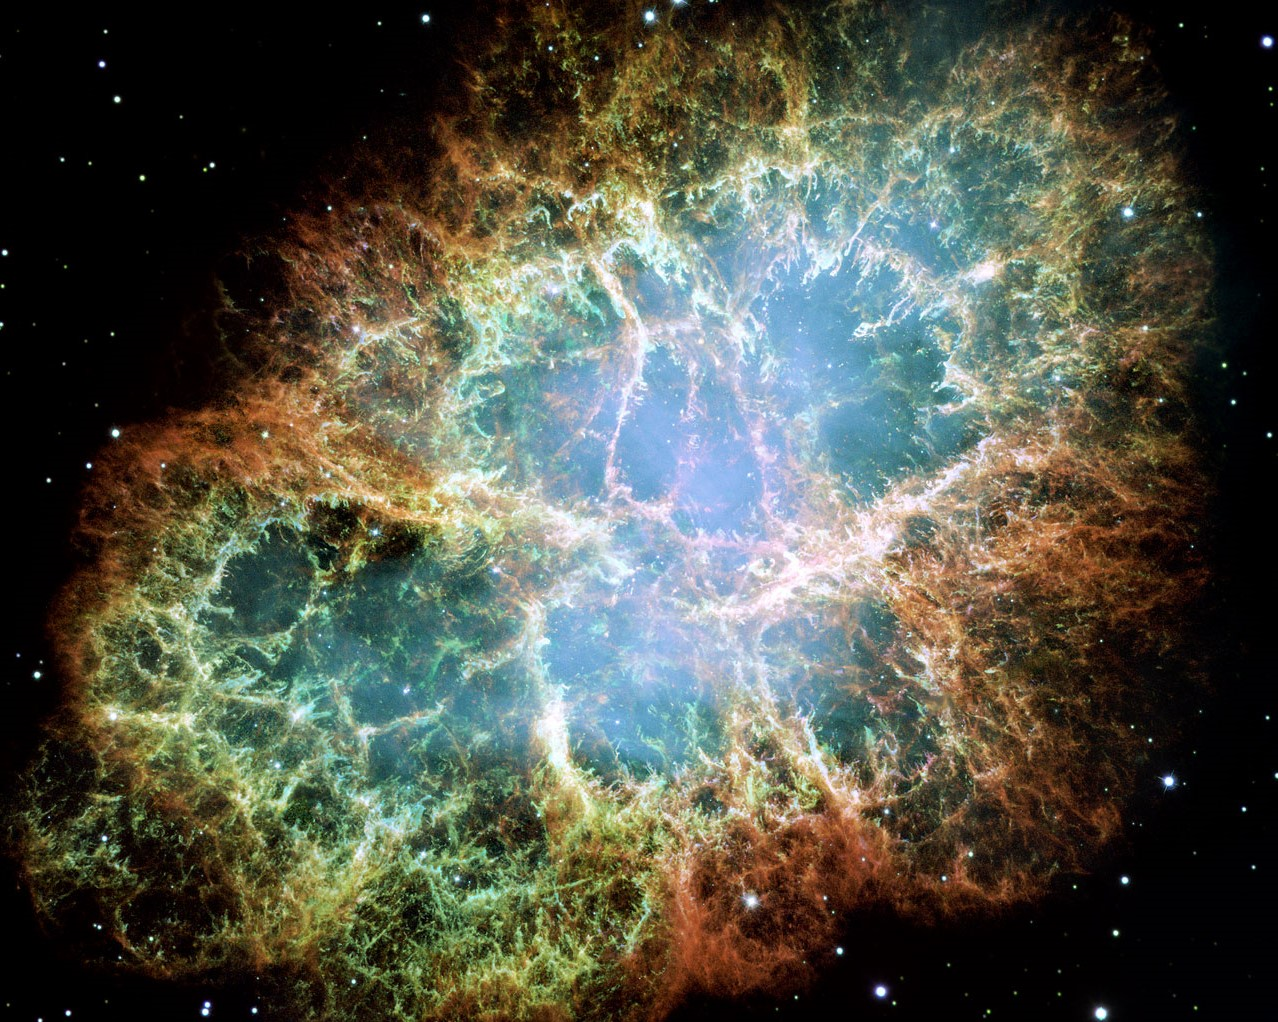
\includegraphics[width=\paperwidth, height =10cm]{../../Crab.jpg}}
    \end{figure}
\end{titlepage}

%%%%%%%%%%%%%%%%%%%%%%%
\tableofcontents

%%%%%%%%%%%%%%%%%%%%%%%%%%%%%%%%%%%%% - Part 1
\part{Vector Space Theory}

%%%%%%%%%%%%%%%%%%%%%% - P1.Chapter 1
%%%%%%%%%% Vector Spaces %%%%%%%%%%
\chapter{Vector Spaces}\label{VecSpaces}
% use \chaptermark{}
% to alter or adjust the chapter heading in the running head

In this chapter we shall build up the basic formulation of abstract linear algebra in terms of vector spaces and their basic formulations.

\section{Vector Space Basics}\label{sec:vecSps}

Before defining a vector space we need the notion of a field.

\begin{definition}\index{Field}
    A triple $(F,+,\cdot)$ of a set $F$ with two binary operations $+:F\times F\rightarrow F$ and $\cdot:F\times F\rightarrow F$ satisfying the following properties is known as a field. \begin{itemize}
        \item The pair $(F,+)$ is an abelian group with identity $0_F$
        \item The pair $(F^*,\cdot)$ is an abelian group with identity $1_F$, with $F^* = F\backslash\{0_F\}$
        \item For any $a,b,c \in F$, the distributive laws hold \begin{equation*}
            a\cdot(b+c) = a\cdot b+a\cdot c,\;\;(b+c)\cdot a = b\cdot a + c\cdot a
        \end{equation*}
    \end{itemize}
\end{definition} 

Moving forward we shall denote a general field by $k$. Now we have the notion of a vector space.

\begin{definition}\index{Vector Space}
    A vector space is a quadruple $(V,+,k,\cdot)$ where $(V,+)$ is an abelian group with identity $0_V$, and $k$ is a field wtih a left field action $\cdot:k\times V\rightarrow V$ known as \textbf{scalar multiplication} satisfying the following properties. For all $a,b \in F$ and all $u,v \in V$ we have distributivity \begin{equation*}
                a\cdot (u+v) = a\cdot u + a \cdot v,\;\; (a+b)\cdot u = a\cdot u + b\cdot u
    \end{equation*}
        associativity \begin{equation*}
            (ab)\cdot u = a\cdot (b\cdot u)
        \end{equation*}
        and identity \begin{equation*}
            1_k\cdot u = u
            \end{equation*}
\end{definition}

The collection of all (small) vector spaces form a category $\Vect$ with maps to be defined in Chapter \ref{LinMaps}. As with all algebraic structures we have the notion of a \textbf{subspace}\index{Subspace} which consists of a subset $U \subseteq V$ which is a vector space under the restrictions of the operations on $V$. We shall write $U \leq V$ to denote a subspace, and $U < V$ to denote a proper subspace.

\begin{example}
    A few common examples of vector spaces and subspaces are as follows. \begin{itemize}
        \item The field $k$ is a vector space over itself with multiplication in place of scalar multiplication.
        \item For any set $X$ and any vector space $V \in \Vect$, the set of functions $V^X$ from $X$ to $V$ inherits a vector space structure from $V$ with pointwise addition and scalar multiplication of functions. A notable subspace is the space $(V^X)_0$ of such functions with finite support.
        \item A special case is the space $V^{\N}$ of all sequences in $V$ and the subspace $(V^{\N})_0$ of all sequences with finite support. For example in $\C^{\N}$ we have the subspace $\ell^{\infty}$ of all bounded complex sequences, or for any $p > 1$ we have the subspace $\ell^p$ of all complex sequences $(z_n)_{n\in\N}$ for which $\left(\sum_{n=1}^{\infty}|z_n|^p\right)^{1/p} < \infty$.
        \item The set $M_{m,n}(k)$ of all $m\times n$ matrices with entries in $k$ is a vector space over $k$ with element wise addition and scalar multiplication.
        \item A special case is the space $k^n = M_{n,1}(k)$ of $n$-tuples whose components lie in $k$.
        \item The polynomial ring $k[X]$ in one indeterminate is a vector space over $k$ with standard addition and multiplication by scalars. It is often denoted $\mathbb{P}(k)$. Additionally, for any $n \in \N$ the space $\mathbb{P}_n(k)$ of polynomials of degree less than or equal to $n$ is a subspace.
    \end{itemize}
\end{example}

Subspaces hold a special structure in vector spaces. If $V \in \Vect$ let $\mathcal{S}(V)$ denote the collection of all subspaces of $V$. Then $\mathcal{S}(V)$ is partially ordered by inclusion and contains both a minimal element $\{0\}$ and a maximal element $V$. In addition, for $S,T \in \mathcal{S}(V)$ the intersection $S\cap T$ forms the largest subspace of $V$ containing both $S$ and $T$, or in other words the greatest lower bound of $S$ and $T$ with respect to inclusion. Similarly, for any family $\{S_{\alpha}\}_{\alpha \in I}$ we can form the intersection $\bigcap_{\alpha \in I}S_{\alpha}$ which is the greatest lower bound of the family. Similarly, we also have a notion of least upper bound formed by \textbf{sums}.

\begin{definition}\index{Sum}
    Let $S,T \leq V$. The \textbf{sum} of $S$ and $T$ is defined to be \begin{equation*}
        S+T := \{u+v|u \in S,v \in T\}
    \end{equation*}
    In general, for a family $\{S_{\alpha}\}_{\alpha \in I}$ the sum is the set of all finite sums of vectors from $\bigcup_{\alpha \in I}S_{\alpha}$: \begin{equation*}
        \sum_{\alpha \in I}S_{\alpha} := \left\{s_{\alpha_1}+\cdots + s_{\alpha_n}\Bigg\vert n \in \N, s_{\alpha_j} \in \bigcup_{\alpha \in I}S_{\alpha}\right\}
    \end{equation*}
\end{definition}

This construction in fact defines the least upper bound of $S$ and $T$ in $\mathcal{S}(V)$, or of $\{S_{\alpha}\}_{\alpha \in I}$ in $\mathcal{S}(V)$ with respect to inclusion. This shows that the collection $\mathcal{S}(V)$ forms a \textbf{lattice} with respect to the partial ordering of inclusion. 

\section{Direct Sums}\label{sec:DirectSum}

We start our journey into vector space constructions with the notion of \textbf{direct sums}.

\begin{definition}\index{External direct sum}
    Let $V_1,...,V_n \in \Vect$. The \textbf{external direct sum} of $V_1,...,V_n$ is the vector space \begin{equation*}
        V_1\boxplus\cdots \boxplus V_n := \{(v_1,...,v_n)|v_i \in V_i,i = 1,...,n\}
    \end{equation*}
    with operations of componentwise addition and scalar multiplication. In general for an index set $I$ and a family of vector space $\{V_{\alpha}\}_{\alpha \in I}$, the direct sum is the space subspace of $(\amalg_{\alpha \in I}V_{\alpha})^I_0$ consisting of functions such that $f(\alpha) \in V_{\alpha}$. We denote this space by \begin{equation*}
        \bigoplus_{\alpha \in I}^{ext}V_{\alpha} = \left\{f:I\rightarrow \amalg_{\alpha \in I}V_{\alpha}\Bigg\vert f(i) \in V_i,f\;\text{has finite support}\right\}
    \end{equation*}
\end{definition}

We also call the subspace of $(\amalg_{\alpha \in I}V_{\alpha})^I$ consisting of all functions such that $f(\alpha) \in V_{\alpha}$ to be the \textbf{direct product} of the family, and denote it by \begin{equation*}
    \prod_{\alpha \in I}V_{\alpha} :=\left\{f:I\rightarrow \amalg_{\alpha \in I}V_{\alpha}\Bigg\vert f(i) \in V_i\right\}
\end{equation*}
In the case that $V_{\alpha} = V \in \Vect$ for all $\alpha$, these spaces are just $(V^I)_0$ and $V^I$ respectively. In the case of $I$ finite we have that these constructions coincide.

Identically to the external direct sum we define the notion of an internal direct sum.

\begin{definition}\Alsoindex{External direct sum}{Internal direct sum}\index{Internal direct sum}
    A vector space $V \in \Vect$ is the \textbf{internal direct sum} of a family $\mathcal{F} = \{S_{\alpha}\}_{\alpha \in I}$ of subspaces of $V$, written \begin{equation*}
        V = \bigoplus \mathcal{F} = \bigoplus_{\alpha \in I}S_{\alpha}
    \end{equation*}
    if the following hold: \begin{itemize}
        \item $V$ is the sum, or join, of the family $\mathcal{F}$: \begin{equation*}
                V = \sum_{\alpha \in I}S_{\alpha}
        \end{equation*}
        \item For each $\alpha \in I$, \begin{equation*}
            S_{\alpha}\cap\left(\sum_{\alpha \neq \beta \in I}S_{\beta}\right) = \{0\}
        \end{equation*}
    \end{itemize}
    In this case each $S_{\alpha}$ is called a direct summand of $V$.
\end{definition}

In the case that $V = S\oplus T$ we say that the subspace $T$ is a \textbf{complement} of $S$ in V.\index{Complement} One should note that a subspace generally has many distinct complements. For example consider lines in $\R^2$ (one-dimensional subspaces). There are also equivalent ways to characterize the independence of a family in a direct sum, as we now show.

\begin{theorem}
    Let $\mathcal{F} = \{S_{\alpha}\}_{\alpha \in I}$ be a family of distinct subspaces of $V$. The following are equivalent: \begin{itemize}
        \item For each $\alpha \in I$, \begin{equation*}
                S_{\alpha}\cap\left(\sum_{\alpha\neq \beta \in I}S_{\beta}\right) = \{0\}
        \end{equation*}
        \item The zero vector $0$ cannot be written as a sum of nonzero vectors from distinct subspaces of $\mathcal{F}$
        \item Every nonzer $v \in V$ has a unique, except for order of terms, expression as a sum $$v = s_1+\cdots + s_n$$
            of nonzero vectors from distinct subspaces in $\mathcal{F}$.
    \end{itemize}
\end{theorem}
\begin{proof}
    First assume the first claim and that the second fails. Then there exist $v_1,...,v_n$ in distinct families which are non-zero and $v_1+\cdots +v_n = 0$. However this implies $-v_1 = v_2+\cdots + v_n$, or $v_1 \in S_{\alpha_1}\cap\left(\sum_{\alpha_1\neq \beta}S_{\beta}\right)$ for $v_1 \neq 0$, contradicting the first claim. 

    Next if the second claim holds and $\sum_{\alpha \in I}s_{\alpha} = \sum_{\alpha \in I}r_{\alpha}$, then $\sum_{\alpha \in I}(s_{\alpha}-r_{\alpha}) = 0$ is an expression of zero in terms of elements of the summands, so $s_{\alpha} = r_{\alpha}$ for each $\alpha \in I$. Finally, if the third claim holds, any non-zero element of $S_{\alpha}$ cannot be written as a sum of elements in $\{S_{\beta}\}_{\beta \neq \alpha}$, so we have that the first statement holds.
\end{proof}


\section{Spans and Linear Independence}\label{sec:SpanLinInd}

We now investigate possibly one of the most central concepts in vector space theory: the notion of spanning and linearly independent sets.

\begin{definition}\index{Span}
    Let $S \subseteq V$ be a nonempty set. We define the span of $S$ to be the set of all linear combinations of vectors from $S$: \begin{equation*}
        \langle S\rangle = \spn(S) = \{r_1v_1+\cdots r_nv_n| n\in \N, r_i \in k,v_i \in S\}
    \end{equation*}
    The set $S$ is said to \textbf{span} or generate $V$ if $V = \spn(S)$. 
\end{definition}

By convention we take $\spn\emptyset = \{0\}$. The span gives us the smallest subspace of $V$ which contains the subset $S$. Next we have the notion of linear independence, relating to minimal generating sets.

\begin{definition}\index{Linearly independence}
    Let $V \in \Vect$. A nonempty set $S \subseteq V$ is \textbf{linearly independent} if for any distinct vectors $s_1,...,s_n \in S$, \begin{equation*}
        a_1s_1+\cdots +a_ns_n = 0\implies a_i = 0,\;\forall i \in \{1,...,n\}
    \end{equation*}
    If $S$ is not linearly independent we say that it is \textbf{linearly dependent}.
\end{definition}

For convenience we consider the emptyset $\emptyset$ to be linearly independent. It is an immediate consequence that a set $S$ is linearly independent if and only if every vector $v \in \spn(S)$ can be expressed uniquely as a linear combination of vectors in $S$, and no vector in $S$ is a linear combination of other vectors in $S$. 

\begin{theorem}
    Let $V \in \Vect$ and let $S \subseteq V$ be linearly independent. If $v \in V$ and $v \notin S$, then $S \cup \{v\}$ is linearly independent if and only if $v \notin \spn(S)$.
\end{theorem}
\begin{proof}
    First if $v \in \spn(S)$ then we could express $v = a_1v_1+\cdots +a_nv_n$ for $v_i \in S$, or in other words $v-a_1v_1-\cdots - a_nv_n = 0$, implying that $S\cup\{v\}$ is not linearly independent. Conversely, if $S \cup \{v\}$ is linearly independent, we have $av+a_1v_1+\cdots +a_nv_n = 0$ for some $a_i \in S$, where $a \neq 0$ since $S$ is linearly independent. Hence $v = -\frac{1}{a}(a_1v_1+\cdots +a_nv_n) \in \spn(S)$.
\end{proof}

Combining linear independence and spanning we arrive at the notion of a basis.

\begin{definition}\index{Basis}
    A subset $\mathcal{B}$ of $V \in \Vect$ is said to be a \textbf{basis} if it is linearly independent and spans $V$.
\end{definition}

Combining with our previous we find equivalently that a every vector in $V$ can be expressed uniquely as a linear combination of vectors in $\mathcal{B}$, $\mathcal{B}$ is a minimal spanning set, and $\mathcal{B}$ is a maximal linearly independent set. Additionally, if $\mathcal{B} = \{v_1,...,v_n\}$ is finite, we can write $V = \langle v_1\rangle \oplus \cdots \oplus \langle v_n\rangle$.

\begin{theorem}
    Let $V \in \Vect$ be a non-zero vector space. Let $I$ be a linearly independent set in $V$ and $S$ a spanning set containing $I$. Then there is a basis $\mathcal{B}$ of $V$ for which $I \subseteq \mathcal{B} \subseteq S$.
\end{theorem}
\begin{proof}
    Let $\mathcal{A}$ denote the collection of all linearly independent subsets of $V$ containing $I$ and contained in $S$. Since $I \in \mathcal{A}$ this is non-empty. Now if $\mathcal{C} = \{I_{\alpha}\}_{\alpha \in J}$ is a chain in $\mathcal{A}$, then the union $U = \bigcup_{\alpha \in J}I_{\alpha}$ is linearly independent and satisfies $I \subseteq U \subseteq S$. Indeed any linear dependence on $U$ would simplify to a linear dependence on an element of $\mathcal{C}$. Hence every chain in $\mathcal{A}$ has an upper bound in $\mathcal{A}$, so by Zorn's lemma $\mathcal{A}$ must contain a maximal element $\mathcal{B}$ which is linearly independent.

    This $\mathcal{B}$ is a basis for $\langle S\rangle = S$, since if any $s \in S$ is not in $\spn(\mathcal{B}$, then $\mathcal{B}\cup\{s\} \subseteq S$ would be a larger linearly independent set, contradicting maximality of $\mathcal{B}$.
\end{proof}

In the case of finite sets we perform an inductive argument. We enumerate $S_1 = S\backslash I = \{v_1,...,v_n\}$. Then if $v_1 \notin \spn(I)$ we form $I_2 = I\cup\{v_1\}$ which is linearly independent and set $S_2 = S_1\backslash\{v_1\}$, and otherwise we simply remove $v_1$. We repeat this process until we arrive at $S_{n+1} = \emptyset$, at which point $I_{n+1}$ is a linearly independent set with equivalent span to $S$.

\begin{theorem}
    If $v_1,...,v_n$ are linearly independent in $V$ and $s_1,...,s_m$ span $V$ then $n \leq m$.
\end{theorem}
\begin{proof}
    First we list the vectors as $s_1,...,s_m;v_1,...,v_n$. Since $s_1,...,s_m$ span $V$, $v_1$ is a linear combination of the $s_i$'s. This implies that there exists $s_i$ which by re-indexing we can choose to be $s_1$ such that $\spn(v_1,s_2,...,s_m) = \spn(s_1,s_2,...,s_m)$. Then $v_1,s_2,...,s_m;v_2,...,v_n$ still represents a spanning and linearly independent set. Now if $m < n$ we can repeat this process to obtain $v_1,...,v_m;v_{m+1},...,v_n$. However, $v_1,...,v_m$ must span $V$ but since $\{v_1,...,v_n\}$ is linearly independent $v_n \notin \spn(v_1,...,v_m)$, which is a contradiction. Hence, $n \leq m$.
\end{proof}

\begin{corollary}
    If $V$ has a finite spanning set, then any two bases of $V$ have the same size.
\end{corollary}

For arbitrary vector spaces we have the following theorem.

\begin{theorem}
    If $V \in \Vect$, then any two bases for $V$ have the same cardinality.
\end{theorem}
\begin{proof}
    We have already covered the finite case, so we may assume all bases of $V$ are infinite. Let $\mathcal{B}$ and $\mathcal{C}$ be bases. Then any vector in $\mathcal{C}$ can be written as a linear combination of vectors in $\mathcal{B}$, and every vector in $\mathcal{B}$ must appear in at least one linear combination as otherwise a proper subset of $\mathcal{B}$ would span $V$. Thus $|\mathcal{B}| \leq \aleph_0|\mathcal{C}| = |\mathcal{C}|$ since the bases are infinite, and reversing the roles we obtain the reverse inequality so $|\mathcal{B}| = |\mathcal{C}|$ by the Schr\"{o}der-Bernstein theorem.
\end{proof}

In the finite dimensional case we find that being a basis of $V$ is equivalent to being a spanning set with size $\dim V$ or a linearly independent set with size $\dim V$.

\begin{theorem}
    If $S \leq V$, then there exists $T \leq V$ such that $V = S\oplus T$.
\end{theorem}
\begin{proof}
    Let $S \leq V$ and let $\mathcal{B}$ be a basis for $S$. As $\mathcal{B}$ is linearly independent in $V$ we can extend it to a basis $\mathcal{B}\cup \mathcal{C}$ of $V$. Let $T = \spn(\mathcal{C})$. By linear independent of $\mathcal{B}\cup\mathcal{C}$ we must have that $S\cap T = \{0\}$, and $V = S+T$ by construction, so $V = S\oplus T$.
\end{proof}

\begin{theorem}
    Let $S,T \leq V \in \Vect$. Then \begin{equation*}
        \dim(S) + \dim(T) = \dim(S+T) + \dim(S\cup T)
    \end{equation*}
\end{theorem}
\begin{proof}
    Suppose $\mathcal{B}$ is a basis for $S\cap T$. Extend this to a basis $\mathcal{A}\cup\mathcal{B}$ for $S$ and a basis $\mathcal{B}\cup\mathcal{C}$ for $T$. We claim $\mathcal{A}\cup\mathcal{B}\cup\mathcal{C}$ is a basis for $S+T$. Evidently it spans $S+T$. To see linear independence suppose to the contrary that we have a linear dependence $\alpha_1v_1+\cdots \alpha_nv_n$ with $\alpha_i \neq 0$ for all $i$. As $\mathcal{A}\cup\mathcal{B}$ and $\mathcal{B}\cup\mathcal{C}$ are linearly independent, this expression must involve elements of $\mathcal{A}$ and $\mathcal{C}$. Isolating the components of $\mathcal{A}$ on one side we have a nonzero vector $x \in \langle \mathcal{A}\rangle \cap\langle \mathcal{B}\cup\mathcal{C}\rangle$. But then $x \in S\cap T$, so $x \in \langle \mathcal{A}\rangle \cap \langle \mathcal{B}\rangle$, which implies $x = 0$, a contradiction. Hence they indeed form a basis for $S+T$, and \begin{equation*}
        \dim(S)+\dim(T) = |\mathcal{A}\cup\mathcal{B}|+|\mathcal{B}\cup\mathcal{C}| = \dim(S+T) + \dim(S\cap T)
    \end{equation*}
\end{proof}


\section{Ordered Bases and Coordinates}\label{sec:coord}

Now that we have a notion of minimal spanning sets which uniquely represent the vectors in a vector space, we can investigate how to represent vector spaces in a canonical fashion. 

\begin{definition}\index{Ordered basis}
    Let $V \in \Vect$ with $\dim V = n \in \N$. An \textbf{ordered basis} for $V$ is an ordered $n$-tuple $(v_1,...,v_n)$ of vectors for which the set $\{v_1,...,v_n\}$ is a basis for $V$.
\end{definition}

If $\mathcal{B} = (v_1,...,v_n)$ is an ordered basis for $V$, then for each $v \in V$ we have a unique ordered $n$-tuple $(r_1,...,r_n)$ of scalars for which $v = r_1v_1+\cdots +r_nv_n$. This defines a bijection known as the \textbf{coordinate map}: $\varphi_{\mathcal{B}}:V\rightarrow k^n$, with $\varphi_{\mathcal{B}}(v) = [v]_{\mathcal{B}} = \begin{bmatrix} r_1 \\ \vdots \\ r_n\end{bmatrix}$. 




%
\section*{Appendices: Constructions}
%
\addcontentsline{toc}{section}{Appendix: Constructions}


%%%%%%%%%%%%%%%%%%%%%% - P1.Chapter 2
%%%%%%%%%% Linear Maps %%%%%%%%%%
\chapter{Linear Maps}




%%%%%%%%%%%%%%%%%%%%%% - P1.Chapter 3
%%%%%%%%%% Matrix Algebra %%%%%%%%%%
\chapter{Matrix Algebra}\label{MatrixAlg}
% use \chaptermark{}
% to alter or adjust the chapter heading in the running head



%%%%%%%%%%%%%%%%%%%%%% - P1.Chapter 4
%%%%%%%%%% Traces and Determinants %%%%%%%%%%
\chapter{Traces and Determinants}



%%%%%%%%%%%%%%%%%%%%%% - P1.Chapter 5
%%%%%%%%%% Spectral Theory %%%%%%%%%%
\chapter{Spectral Theory}



%%%%%%%%%%%%%%%%%%%%%% - P1.Chapter 6
%%%%%%%%%% Canonical Forms %%%%%%%%%%
\chapter{Canonical Forms}\label{CanonicalForms}
% use \chaptermark{}
% to alter or adjust the chapter heading in the running head

This chapter aims to investigate the canonical forms of linear operators on finite dimensional vector spaces. A canonical form for linear operators $\mathcal{L}(V,W)$ is a collection of representatives for some equivalence relation on $\mathcal{L}(V,W)$, such that we only have one representative for each equivalence class. Some of the constructions in this chapter follow from results on module theory over PIDs which is discussed in Chapter \ref{PIDMod}. We begin by investigating the general form for operators in $\mathcal{L}(V,W)$ known as the Singular Value Decomposition.

\section{Singular Value Decomposition}\label{sec:SVD}

\begin{theorem}[Singular Value Decomposition]\index{Singular Value Decomposition}
    Let $V$ and $W$ be finite dimensional inner product spaces over $k$ ($= \C$ or $\R$) and let $\tau \in \mathcal{L}(V,W)$ have rank $r$. Then there are ordered orthonormal bases $\mathcal{B}$ and $\mathcal{C}$ for $V$ and $W$, respectively, for which $\mathcal{B} = (u_1,..,u_r,u_{r+1},...,u_n)$ where up to $r$ is an ONB of $\ran(\tau^*)$ and from $r+1$ to $n$ is an ONB for $\ker(\tau)$, and where $\mathcal{C} = (v_1,...,v_r,v_{r+1},...,v_m)$ with the vectors up to $r$ being an ONB for $\ran(\tau)$ and the vectors from $r+1$ to $m$ being an ONB for $\ker(\tau^*)$. Moreover, for $1 \leq k \leq r$, \begin{equation*}
        \tau u_i = s_iv_i,\;\;\tau^*v_i = s_iu_i
    \end{equation*}
    where $s_i > 0$ are called the \textbf{singular values} of $\tau$ and defined by $\tau^*\tau u_i = s_i^2u_i,s_i > 0$ for $i \leq r$.
\end{theorem}
\begin{proof}
    First observe that $\tau^*\tau$ is self-adjoint and positive definite. Additionally $r = \text{rank}(\tau) = \text{rank}(\tau^*\tau)$, and by the spectral theorems $V$ has an ordered orthonormal basis $\mathcal{B} = (u_1,...,u_r,u_{r+1},...,r_n)$ of eigenvectors for $\tau^*\tau$, where the corresponding eigenvalues can be arranged so that $\lambda_1\geq \cdots \geq \lambda_r > 0 = \lambda_{r+1}=\cdots = \lambda_n$. The set $(u_{r+1},...,u_n)$ is an ONB for $\ker(\tau^*\tau) = \ker(\tau)$, and so $(u_1,...,u_r)$ is an ONB for $\ker(\tau)^{\perp} = \ran(\tau^*)$. For $i = 1,...,r$, the positive numbers $s_i = \sqrt{\lambda_i}$ are called the \textbf{singular values} of $\tau$. If we set $s_i = 0$ for $i > r$, then $\tau^*\tau u_i = s_i^2u_i$ for $i = 1,...,n$. Set $v_i = (1/s_i)\tau u_i$ for each $i \leq r$, so $\tau u_i = s_iv_i$ for $i \leq r$, and $\tau^*v_i = s_iu_i$ for $i \leq r$. The vectors $v_1,...,v_r$ are orthonormal, since if $i,j \leq r$, then \begin{equation*}
        \langle v_i,v_j\rangle = \frac{1}{s_is_j}\langle \tau u_i,\tau u_j\rangle = \frac{1}{s_is_j}\langle \tau^*\tau u_i,u_j\rangle = \frac{s_i}{s_j}\langle u_i,u_j\rangle = \delta_{i,j}
    \end{equation*}
    Hence $(v_1,...,v_r)$ is an orthonormal basis for $\ran(\tau) = \ker(\tau^*)^{\perp}$, which can be extended to an orthonormal basis $\mathcal{C} = (v_1,...,v_m)$ for $v$, with the extension $(v_{r+1},...,v_m)$ being an orthonormal basis for $\ker(\tau^*)$. Moreover, since $\tau\tau^*v_i = s_i\tau u_i = s_i^2v_i$, the vectors $v_1,...,v_r$ are eigenvectors for $\tau\tau^*$ with the same eigenvalues $\lambda_i = s_i^2$ as for $\tau^*\tau$. This completes the proof.
\end{proof}

Writing this result in the language of matrices gives the following decomposition.

\begin{corollary}[Singular Value Decomposition]
    If $A \in M_{m,n}(k)$ of rank $r$ then there exists an $n\times n$ unitary matrix $Q = [q_1\;q_2\;\cdots \;q_n]$ where the columns of $Q$ are eigenvectors of $A^*A$ ordered in decreasing eigenvalue $\lambda_1 \geq \cdots \geq \lambda_r > 0 = \lambda_{r+1}=\cdots = \lambda_n$, where $p_1 = \frac{1}{\sqrt{\lambda_1}}Aq_1,...,p_r = \frac{1}{\sqrt{\lambda_r}}Aq_r$ forms an orthonormal basis for $\ran(A)$, and extending it to an orthonormal basis of $k^m$, $p_1,...,p_m$, the matrix $P = [p_1\;\cdots \;p_m]$ is unitary. Finally, we have that \begin{equation*}
        P^*AQ = \sum = \left[\begin{array}{c|c} \begin{array}{ccc} \sqrt{\lambda_1} &  &  \\  & \ddots &  \\  &  & \sqrt{\lambda_r} \end{array} & \mathbf{0} \\ \hline \mathbf{0} & \mathbf{0} \end{array}\right]
    \end{equation*}
\end{corollary}


\section{Eigenspaces and Diagonalization}\label{sec:Eigen}

Next we investigate a special form for square matrices. However, this form is not canonical as it is too restrictive, so not every equivalence class has a diagonal representative. 

To discuss the notion of diagaonalization we note that having a diagonal basis is equivalent to having a basis for which our operator acts by scaling on each vector.

\begin{definition}\index{Eigenvalue}\index{Eigenvector}
    Let $V \in \Vect$ and $\tau \in \mathcal{L}(V)$. A scalar $\lambda \in k$ is called an \textbf{eigenvalue} of $\tau$ if there exists a nonzero vector $v \in V$ for which $\tau v = \lambda v$. In this case $v$ is called an \textbf{eigenvector} of $\tau$ with associated eigenvalue $\lambda$. The collection of all eigenvectors associated with $\lambda$, together with $0$, forms a subspace of $V$ called the \textbf{eigenspace} of $\lambda$ and denoted by $E_{\lambda}$. The collection of all eigenvalues of $\tau$ is called its \textbf{spectrum}.
\end{definition}

We have the following result.

\begin{theorem}
    Let $\tau \in \mathcal{L}(V)$. A scalar $\lambda \in k$ is an eigenvalue of $\tau$ if and only if $\tau - \lambda I_V$ is singular.
\end{theorem}

Thus we can find the eigenvalues of an operator by finding the roots of the \textbf{characteristic polynomial} given by $c_{\tau}(\lambda) = \det(\tau-\lambda I_V)$, where we take any matrix representation of the transformation.

\begin{theorem}
    Suppose $\lambda_1,...,\lambda_k \in \text{Spec}(\tau)$ are distinct eigenvalues of a linear operator $\tau \in \mathcal{L}(V)$. Then if $v_i \in E_{\lambda_i}$ are non-zero eigenvectors, $\{v_1,...,v_k\}$ are linearly independent.
\end{theorem}
\begin{proof}
    Suppose we have a linear relation of minimal size $r_1v_1+\cdots+r_jv_j = 0$. Applying $\tau$ to both sides $r_1\lambda_1v_1+\cdots+r_j\lambda_jv_j = 0$. Subtracting $\lambda_1$ times the first equation from the second, $r_2(\lambda_2-\lambda_1)v_2+\cdots+r_j(\lambda_j-\lambda_1)v_j = 0$. This is a smaller linear relation, contradicting minimality, so we must have that $\{v_1,...,v_k\}$ is linearly independent.
\end{proof}

Since the eigenvalues of $\tau$ are given by the roots of a polynomial of order $\dim V$, $\tau$ has at most $\dim V$ eigenvalues. This can also be seen using the previous theorem and the uniqueness of the dimension of a space.

\begin{corollary}
    Let $V \in \Vect$. If $\lambda_1,...,\lambda_k$ are pairwise distinct eigenvalues of $\tau \in \mathcal{L}(V)$, then the sum $E_{\lambda_1}+\cdots+E_{\lambda_k}$ is direct.
\end{corollary}

We can now characterize diagonalizability of operators.

\begin{theorem}
    Let $V \in \Vect$, $\dim V = n \in \N$, and let $\tau \in \mathcal{L}(V)$. Then $T$ is diagonalizable if and only if $V = \bigoplus_{\lambda \in \text{Spec}(\tau)}E_{\lambda}$.
\end{theorem}

\begin{definition}\index{Algebraic multiplicity}
    Let $V \in \Vect, \dim V = n\in \N$. Let $\tau \in \mathcal{L}(V)$ and $\lambda$ a root of $c_{\tau}(t)$. Then the \textbf{algebraic multiplicity of} $\lambda$ is the largest positive integer $k$ such that $c_{\tau}(t) = (t-\lambda)^kq(t)$ with $q(\lambda) \neq 0$.
\end{definition}

\begin{theorem}
    Let $V \in \Vect, \dim V = n \in \N$ and let $\tau \in \mathcal{L}(V)$. If $\lambda \in \text{Spec}(\tau)$ with algebraic multiplicity $k$, then $1 \leq \dim(E_{\lambda}) \leq k$.
\end{theorem}
\begin{proof}
    Since $\lambda$ is an eigenvalue of $\tau$, $\dim(E_{\lambda}) \geq 1$. Now let $\{v_1,...,v_p\}$ be a basis of $E_{\lambda}$ and extend it into a basis $\mathcal{B}$ of $V$. Then \begin{equation*}
        [\tau]_{\mathcal{B}}^{\mathcal{B}} = \left[\begin{array}{c|c} \begin{array}{ccc} \lambda & & \\ & \ddots & \\ & & \lambda \end{array} & \mathbf{A} \\ \mathbf{0} & \mathbf{B} \end{array}\right]
    \end{equation*}
    so $c_{\tau}(t) = (t-\lambda)^pc_{\mathbf{B}}(t)$. Thus we must have that $p \leq k$, so $\dim(E_{\lambda}) \leq k$.
\end{proof}

\begin{definition}
    Let $\tau \in \mathcal{L}(V)$ and $\lambda \in \text{Spec}(\tau)$. Then $\dim(E_{\lambda})$ is called the \textbf{geometric multiplicity} of $\lambda$.
\end{definition}

We then have the following result.

\begin{theorem}
    Let $V \in \Vect, \dim V = n\in \N$, and let $\tau \in \mathcal{L}(V)$. Then $\tau$ is diagonalizable if and only if for all $\lambda \in \text{Spec}(\tau)$, $\dim(E_{\lambda}) = $ the algebraic multiplicity of $\lambda$.
\end{theorem}

\subsection{Invariant Subspaces}

\begin{definition}\index{Invariant subspace}
    Let $V \in \Vect$ and $\tau \in \mathcal{L}(V)$. A subspace $U \leq V$ is said to be \textbf{invariant under} $\tau$ or $\tau$-\textbf{invariant} if $\tau(U) \subseteq U$.
\end{definition}

This means that $\tau$ restricts to a linear operator on $U$, or $\tau\vert_U \in \mathcal{L}(U)$. 

\begin{theorem}
    Let $V \in\Vect, \dim V =n\in\N$ and let $\tau \in \mathcal{L}(V)$. If $U \leq V$ is $\tau$-invariant, then the characteristic polynomial of $\tau\vert_U$ divides the characteristic polynomial of $\tau$.
\end{theorem}
\begin{proof}
    Let $\beta = \{u_1,...,u_m\}$ be a basis of $U$ and extend to a basis $\mathcal{B} = \{u_1,...,u_m,v_{m+1},...,v_n\}$ of $V$. Then \begin{equation*}
        [\tau]_{\mathcal{B}} = \begin{bmatrix} [\tau\vert_U]_{\beta} & \mathbf{A} \\ \mathbf{0} & \mathbf{B} \end{bmatrix}
    \end{equation*}
    so $c_{\tau}(t) = c_{\tau\vert_U}(t)c_{\mathbf{B}}(t)$, as desired.
\end{proof}

\begin{corollary}
    Let $V \in \Vect,\dim V = n\in\N$ and $\tau \in \mathcal{L}(V)$. If $V = U_1\oplus \cdots \oplus U_k$ for $\tau$-invariant subspaces $U_i$, then we have that \begin{equation*}
        c_{\tau}(t) = \prod_{i=1}^kc_{\tau\vert_{U_i}}(t)
    \end{equation*}
\end{corollary}

We have the following important result which shall be used in deriving our next canonical form.

\begin{theorem}
    Let $V \in \Vect, \dim V = n\in\N$ and let $\tau \in \mathcal{L}(V)$. For $u \in V\backslash\{0\}$ let $U = \spn(u,\tau u,\tau^2u,...)$. Then $\dim(U) = k \leq n$, and we have \begin{itemize}
        \item $\{u,\tau u,...,\tau^{k-1}u\}$ is a basis of $U$
        \item $U$ is $\tau$-invariant
        \item $U$ is the smallest invariant subspace of $V$ that contains $u$
        \item If $a_0,a_1,...,a_{k-1} \in k$ such that $a_0u+a_1\tau u+\cdots +a_{k-1}\tau^{k-1}u+\tau^ku = 0$, then $c_{\tau\vert_U}(t) = a_0+a_1t+\cdots+a_{k-1}t^{k-1}+t^k$.
    \end{itemize}
\end{theorem}
\begin{proof}
    First let $k\in \N$ be the largest integer for which $\{u,\tau u,...,\tau^{k-1}u\}$ is linearly independent. Since $\dim V = n$ $k$ exists and is $\leq n$, and as $u\neq 0$, $k \geq 1$. It follows that $\tau^ku \in \spn(u,\tau u,...,\tau^{k-1}u)$, and so if $\tau^{k+l}u = \sum_{i=0}^{k-1}a_i\tau^iu$ for some $l \geq 0$, $\tau^{k+l+1}u = \sum_{i=0}^{k-1}a_i\tau^{i+1}u \in \spn(u,\tau u,...,\tau^{k-1}u)$. Hence $U \subseteq \spn(u,\tau u,...,\tau^{k-1}u)\subseteq U$, so $\mathcal{B} = \{u,\tau u,...,\tau^{k-1}u\}$ is a basis for $U$. By construction $U$ is $\tau$ invariant and the smallest subspace of $V$ that contains $u$ and is $\tau$-invariant. As $\tau^ku \in \spn(u,\tau u,...,\tau^{k-1}u)$, there exist unique $a_0,...,a_{k-1} \in k$ such that $a_0u+a_1\tau u+\cdots +a_{k-1}\tau^{k-1}u + \tau^ku = 0$. Now we have the matrix representation \begin{equation*}
        [\tau\vert_U]_{\mathcal{B}} = \begin{bmatrix} 0 & 0 & 0 & \cdots & -a_1 \\ 1 & 0 & 0 & \cdots & -a_2 \\ 0 & 1 & 0 & \cdots & -a_3 \\ \vdots & \vdots & \ddots & \ddots & \vdots \\ 0 & 0 & \cdots & 1 & -a_{k-1} \end{bmatrix}
    \end{equation*}
    so $c_{\tau\vert_U}(t) = a_0+a_1t+\cdots+a_{k-1}t^{k-1}+t^k$.
\end{proof}

We then obtain the following well known result.

\begin{theorem}[Cayley-Hamilton]\index{Cayley-Hamilton Theorem}
    Let $V \in \Vect,\dim V = n\in \N$, and let $\tau \in \mathcal{L}(V)$. Then $c_{\tau}(\tau) = 0 \in \mathcal{L}(V)$.
\end{theorem}

This result follows from the previous theorem and our result that the characteristic polynomial of inveriant subspaces divides the characteristic polynomial of the operator.


\section{Jordan Canonical Form}\label{sec:Jord}

Now we lessen the condition of diagonalization to obtain a true canonical form. In order to derive this form we introudce the notion of a generalized eigenvector.

\begin{definition}\index{Generalized eigenvector}
    Let $V \in \Vect$ and $\tau \in \mathcal{L}(V)$ with $\lambda \in \text{Spec}(\tau)$. A nonzero vector $v \in V$ is said to be a \textbf{generalized eigenvector} of $\tau$ associated with $\lambda$ if there exists $k \geq 1$ such that $(\tau-\lambda \id_V)^kv = 0$ and $(\tau - \lambda \id_V)^{k-1}v \neq 0$. $k$ is called the \textbf{index} of the generalized eigenvector $v$.
\end{definition}

Note eigenvectors are generalized eigenvectors of index $1$, and in general $(\tau-\lambda I)^{k-1}v$ is an eigenvector of $\tau$ associated with $\lambda$. To show a vector $v \in V$, $v\neq 0$, is a generalized eigenvector of $\tau$ associated with $\lambda$, it sufficies to show that $(\tau - \lambda \id_V)^mv = 0$ for some $m \geq 1$. Now, from our previous result we know $U = \spn(u,(\tau - \lambda \id_V)v,...)$ is a $\tau$-invariant subspace with basis $u,(\tau-\lambda \id_V)u,...,(\tau-\lambda\id_V)^{k-1}u$. We now define the generalized eigenspace.

\begin{definition}
    Let $\tau \in \mathcal{L}(V)$ and $\lambda \in \text{Spec}(\tau)$. We define the \textbf{generalized eigenspace} of $\lambda$ to be $G_{\lambda}$ which consists of all generalized eigenvectors as well as $v = 0$.
\end{definition}

If $r$ is the largest index of all generalized eigenvectors in $G_{\lambda}$, $G_{\lambda} = \ker (\tau - \lambda \id_V)^r$. As $r \leq n$ by our previous result and the fact that $\dim V = n$, we have always that $G_{\lambda} = \ker (\tau - \lambda \id_V)^n$. 

\begin{definition}
    The largest index $r$ of all generalized eigenvectors in $G_{\lambda}$ is called the \textbf{index} of $G_{\lambda}$.  
\end{definition}

Although eigenspaces often were of insufficient dimension to give a full basis of the space, this issue doesn't arise anymore for generalized eigenspaces. We show this after showing we can construct bases of a particular type.

\begin{theorem}
    Let $V \in \Vect,\dim V = n\in \N$ and $N \in \mathcal{L}(V)$ a nilpotent operator. Then there exists a basis $\{N^{k_1}v_1,...,Nv_1,v_1,...,N^{k_j}v_j,...,Nv_j,v_j\}$ of $V$.
\end{theorem}
\begin{proof}
    We proceed by induction on the dimension $n$ of $V$. If $n = 1$ then taking any nonzero $v_1$ gives a basis $\{v_1\}$ of $V$. Suppose the claim holds for all dimensions $< n$. Then as $N$ is nilpotent $\dim(\ran N) < n$, so there exists a basis $\{N^{k_1}v_1,...,Nv_1,v_1,...,N^{k_j}v_j,...,Nv_j,v_j\}$ of $\ran N$. Then there exists $u_1,...,u_j$ such that $Nu_i = v_i$, so $\mathcal{A} = \{N^{k_1+1}u_1,...,Nu_1,u_1,...,N^{k_j+1}u_j,...,Nu_j,u_j\}$ is a linearly independent set in $V$. We extend to a basis of $V$ by adding $w_{j+1},...,w_m$. As $Nw_i \in \ran N$ there exists $v_i \in \spn(\mathcal{A})$ such that $Nw_i = Nv_i$. Letting $u_i = w_i-v_i \notin \spn(\mathcal{A})$ as $w_i \notin \spn(\mathcal{A})$, we have our desired basis \begin{equation*}
        \{N^{k_1+1}u_1,...,Nu_1,u_1,...,N^{k_j+1}u_j,...,Nu_j,u_j,u_{j+1},...,u_m\}
    \end{equation*}
\end{proof}


\begin{theorem}
    Let $V \in \Vect,\dim V = n\in \N$ and $\tau \in \mathcal{L}(V)$. Let $\lambda \in\text{Spec}(\tau)$ with algebraic multiplicity $m$. Then $\dim(G_{\lambda}) = m$.
\end{theorem}
\begin{proof}
    First note that $\tau\vert_{G_{\lambda}}$ is a nilpotent mapping, so by the previous theorem we have a basis $\{(\tau-\lambda\id_V)^{k_1}v_1,...,(\tau-\lambda\id_V)v_1,v_1,...,(\tau-\lambda\id_V)^{k_j}v_j,...,(\tau-\lambda\id_V)v_j,v_j\}$ of $G_{\lambda}$. Now, as both are terminal in their respective sequences, $\ker(\tau-\lambda\id_V)^n\cap\ran(\tau-\lambda\id_V)^n = \{0\}$, so by the dimension theorem $V = G_{\lambda}\oplus \ran(\tau-\lambda\id_V)^n$, both of which are $\tau$-invariant. Then we can extend this to a basis $\mathcal{B}$ of $V$ with a basis of $\ran(\tau-\lambda \id_V)^n$. Then the associated matrix representation is \begin{equation*}
        [\tau]_{\mathcal{B}} = \left[\begin{array}{c|c} \text{diag}(J_{k_1}(\lambda),...,J_{k_j}(\lambda)) & \mathbf{0} \\ \mathbf{0} & \mathbf{A}\end{array}\right]
    \end{equation*}
    where $J_k(\lambda) = \begin{bmatrix} \lambda & 1 & 0&  \cdots & 0 \\ 0 & \lambda & 1 & \cdots & 0 \\ \vdots & \vdots & \ddots & \ddots & \vdots \\ 0 & \cdots & 0 & \lambda & 1 \\ 0 & \cdots & 0 & 0 & \lambda \end{bmatrix}$ is the \textbf{Jordan block of size $k$}. Then $c_{\tau}(t) = (t-\lambda)^{\dim G_{\lambda}}c_{\mathbf{A}}(t)$. As $G_{\lambda}\cap \ran(\tau-\lambda\id_V)^n = \{0\}$ and all $\lambda$ eigenvectors are in $G_{\lambda}$, we must have that $c_{\mathbf{A}}(\lambda) \neq 0$. Hence, $\dim G_{\lambda} = m$ must be the algebraic multiplicity of $\lambda$.
\end{proof}

We now have a type of spectral theorem for generalized eigenspaces.

\begin{theorem}
    Let $V\in\Vect, \dim V = n\in \N$ be a vector space over an algebraically closed field $k$. Let $\tau \in \mathcal{L}(V)$ and let $\lambda_1,...,\lambda_k$ be the distinct eigenvalues of $T$ with multiplicities $n_1,...,n_k$. Then $V = G_{\lambda_1}\oplus\cdots\oplus G_{\lambda_k}$.
\end{theorem}
\begin{proof}
    By the previous theorem it is sufficient to show that for $v_1 \in G_{\lambda_1},...,v_k \in G_{\lambda_k}$, not all zero, $v_1+\cdots + v_k \neq 0$. Towards a contradiction suppose $v_1+\cdots+v_k = 0$. Without loss of generality we may suppose $v_1 \neq 0$, and that $v_1$ has index $k_1$, and in general $v_i$ has index $k_i$. Then if $(\tau-\lambda_1\id_V)^{k_1-1}v_1 = w \neq 0$, $\tau w = \lambda_1 w$, so $\prod_{i=2}^{k}(\tau-\lambda_i\id_V)^{k_i}w = \prod_{i=1}^2(\lambda_1-\lambda_i)^{k_i}w \neq 0$. However, $0 = (\tau-\lambda_1\id_V)^{k_1-1}\prod_{i=2}^{k}(\tau-\lambda_i\id_V)^{k_i}(v_1+\cdots+v_k) = \prod_{i=1}^2(\lambda_1-\lambda_i)^{k_i}w$, which is a contradiction. Hence the generalized eigenspaces must be linearly independent. Hence, as $\dim(G_{\lambda_i}) = n_i$ from the previous result, and $n_1+\cdots+n_k = n$, we have that $$V=\bigoplus_{i=1}^kG_{\lambda_i}$$
\end{proof}

The bases with Jordan blocks we used in the previous proofs is known as the \textbf{Jordan canonical basis} of $\tau$, and gives the Jordan canonical form when the operator is represented in that basis.

\begin{definition}
    Let $V \in \Vect$ and $\tau \in \mathcal{L}(V)$. Let $v \in G_{\lambda}\backslash\{0\}$ for $\lambda \in \text{Spec}(\tau)$. Let $k \geq 1$ be the index of $v$. Then we call the ordered linearly independent set $\{(\tau-\lambda \id_V)^{k-1}v,...,(\tau-\lambda\id_V)v,v\}$ is called a \textbf{cycle} of generalized eigenvectors of $\tau$ associated with the eigenvalue $\lambda$. $(\tau-\lambda\id_V)^{k-1}v$ is called the \textbf{initial vector} of the cycle and $v$ is called the \textbf{end vector} of the cycle. $k$ is called the \textbf{length} of the cycle.
\end{definition}

Note that the number of Jordan blocks total is given by the number of linearly independent eigenvectors, since all cycles must end in an eigenvector. The next result gives how to determine the number of blocks of any size.


\begin{theorem}
    Let $\tau \in \mathcal{L}(V)$ for $\dim V = n$. Let $k_j = \dim(\ker(\tau-\lambda\id_V)^j)$. Then the number of Jordan blocks of eigenvalue $\lambda$ of size $j$ is given by $$m_j = 2k_j - k_{j+1}-k_{j-1}$$
\end{theorem}
\begin{proof}
    First I claim that there are $k_{j+1}-k_j$ Jordan blocks of size $> j$. As each Jordan block of size $> j$ will contribute $+1$ to the dimension of $k_{j+1}$ versus $k_j$, $k_{j+1}-k_j$ must be the number of Jordan blocks of size $> j$. Thus, the number of Jordan blocks of size exactly $j$ is $k_j - k_{j-1} - (k_{j+1} - k_j) = 2k_j - k_{j-1} - k_{j+1}$.
\end{proof}

Then we have the following algorithm for determining the Jordan canonical basis of an operator $\tau \in \mathcal{L}(V)$: 

\begin{itemize}
    \item[(1)] Find the value minimal $k$ for which $\ker(\tau-\lambda \id_V)^k = G_{\lambda}$
    \item[(2)] Find a basis $(v_k^1,...,v_k^{m_k})$ of the subspace of $\ker(\tau-\lambda\id_V)^k$ not including $\ker(\tau-\lambda\id_V)^{k-1}$, where $m_k = k_k-k_{k-1}$
    \item[(3)] If $k = 1$, stop, Else, apply $(\tau - \lambda\id_V)$ to the vectors from the previous part. Extend $((\tau-\lambda \id_V)v_k^1,...,(\tau-\lambda\id_V)v_k^{m_k})$ to a basis of $\ker(\tau-\lambda\id_V)^{k-1}$ not including $\ker(\tau-\lambda\id_V)^{k-2}$.
    \item[(4)] Repeat step (3) replacing $k$ with $k-1$ until we hit $k = 1$.
\end{itemize}






%%%%%%%%%%%%%%%%%%%%%% - P1.Chapter 7
%%%%%%%%%% Inner Product Spaces %%%%%%%%%%
\chapter{Inner Product Spaces}


%%%%%%%%%%%%%%%%%%%%%%%%%%%%%%%%%% Part 2
\part{Module Theory}

%%%%%%%%%%%%%%%%%%%%%% - P2.Chapter 1
%%%%%%%%%% Free Modules %%%%%%%%%%
\chapter{Free Modules}



%%%%%%%%%%%%%%%%%%%%%% - P2.Chapter 2
%%%%%%%%%% Linear Transformations %%%%%%%%%%
\chapter{Linear Transformations}


%%%%%%%%%%%%%%%%%%%%%% - P2.Chapter 3
%%%%%%%%%% Module Matrix Theorey %%%%%%%%%%
\chapter{Matrix Theory Over Free Modules}



%%%%%%%%%%%%%%%%%%%%%% - P2.Chapter 4
%%%%%%%%%% PIDs %%%%%%%%%
\chapter{ Principal Ideal Domains}
\label{PIDs}
% use \chaptermark{}
% to alter or adjust the chapter heading in the running head
\section{ Basic Definitions and Examples: PIDs}

\begin{definition}
    An integral domain of which every ideal is principal is called a \Emph{principal ideal domain} (\Emph{PID}).
\end{definition}

\begin{remark}
    $\Z$ is a prototypical example of a PID. Additionally, for a field $\F$, $\F[X]$ is also a PID.
\end{remark}

\begin{theorem}
    Let $\F$ be a field. Then $\F[X]$ is a principal ideal domain. Moreover, every non-zero ideal $I$ of $\F[X]$ is generated by the monic polynomial of lowest degree in $I$.
\end{theorem}
\begin{proof}
    Note that since $\F$ is an integral domain so is $\F[X]$. Consider an ideal $I \subseteq \F[X]$. If $I = \{0\} = (0)$ we are done, so assume $I \neq \{0\}$ and that $0 \neq g \in I$ is of minimal degree. We can assume that $g$ is monic; if $a$ is the leading coefficient of $g$, then $a^{-1} \in \F$ so $a^{-1}g$ is monic, and we replace $g$ with $a^{-1}g \in I$ since $I$ is an ideal. We claim that $I = (g)$. Since $g \in I$ and $I$ is an ideal we have $g\F[X] = (g) \subseteq I$. Let $P \in I$. By the division algorithm there exist unique $q,r \in \F[X]$ such that $P = qg + r$ where $r = 0$ or $\deg(r) < \deg(g)$ since the leading coefficient of $g$ is a unit. Then $r = P - qg \in I$ since $qg \in I$ as it is an ideal. Then $r = 0$, since otherwise $\deg(r) < \deg(g)$, contradicting the minimality of $g$'s degree. Thus, $P = qg \in (g)$, so $I \subseteq (g)$. Therefore $I = (g)$ and $\F[X]$ is a PID as claimed.
\end{proof}




%%%%%%%%%%%%%%%%%%%%%%%%%%%%%%%%%% Part 3
\part{Multilinear Algebra}


%%%%%%%%%%%%%%%%%%%%%% - P3.Chapter 1
%%%%%%%%%% Tensor Products %%%%%%%%%%
\chapter{Tensor Products}\label{Tensors}
% use \chaptermark{}
% to alter or adjust the chapter heading in the running head


%%%%%%%%%%%%%%%%%%%%%% - Appendices
%%%%%%%%%% APPENDIX %%%%%%%%%%
\begin{appendices}
    \section{Important Algebraic Structures}
    
    
    \section{Euclidean Space and Geometry}
\end{appendices}


\end{document}


%%%%%% END %%%%%%%%%%%%%u
